\chapter{Example Configuration File}
\label{chapter:appendixB}

\vspace{9.5cm}


\begin{lstlisting}[caption={Excerpt of the Facial Expression Mimicry \textit{Effector} configuration file. The final animation is the \texttt{BaseAnimation} appended with a random number between 1 and 5, resulting on, for example, suprise3.},label={lst:facialExpressionsSettings},language=XML]
<MimicFacialExpressionsSettings>
  <MinimumMimicDelay>3500</MinimumMimicDelay>
  <Happy>
    <Probability>0.5</Probability>
    <MinimumIntensity>0.65</MinimumIntensity>
    <Priority>1</Priority>
    <BaseAnimation>joy</BaseAnimation>
  </Happy>
  <Sad>
    <Probability>0.5</Probability>
    <MinimumIntensity>0.65</MinimumIntensity>
    <Priority>1</Priority>
    <BaseAnimation>sadness</BaseAnimation>
  </Sad>
  <Surprised>
    <Probability>0.5</Probability>
    <MinimumIntensity>0.5</MinimumIntensity>
    <Priority>1</Priority>
    <BaseAnimation>surprise</BaseAnimation>
  </Surprised>
</MimicFacialExpressionsSettings>
\end{lstlisting}

\chapter{Example \textit{Effector} Plugin}

\vspace{9.5cm}

\begin{lstlisting}[language=CSharp, caption={Example definition of an \textit{Effector} Plugin that mimics facial expressions using event handlers.},classoffset=2,morekeywords={RenderState,PrimitiveRestart,FacetCulling,RasterizationMode,ScissorTest,StencilTest,DepthTest,DepthRange,Blending,ColorMask},label={lst:facialExpressionsSourceCode}]
using GRETAConnection;
using RapportActionProposer.ProposeStrategies;
using RapportActionProposer.RCPluginDefinition;
using RapportAgentPlugin;
using System;
using System.ComponentModel.Composition;

namespace MimicFacialExpressions {

    public class MimicFacialExpressionsSettings {
        public class ExpressionTriggerSetting {
            public double TriggerProbability { get; set; } = 0.48;
            public double MinimumIntensity { get; set; }
            public ushort Priority { get; set; }
            public string BaseAnimation { get; set; }
        }
        
        public int MinimumDelayMsBetweenActions { get; set; } = 3500;
        
        public ExpressionTriggerSetting Happy { get; set; } = new ExpressionTriggerSetting() 
            { MinimumIntensity = 0.65, Priority = 1, BaseAnimation = "joy" };

        public ExpressionTriggerSetting Sad { get; set; } = new ExpressionTriggerSetting() 
            { MinimumIntensity = 0.65, Priority = 1, BaseAnimation = "sadness"};

        public ExpressionTriggerSetting Surprised { get; set; } = new ExpressionTriggerSetting() 
            { MinimumIntensity = 0.5, Priority = 1, BaseAnimation="surprise" };
    }

    [Export(typeof(IRCPlugin))]
    [RCPluginMetadata(Description = "Mimics human emotions")]
    [EffectorMetadata(ProposalsManagementStrategy = ProposeStrategyType.OneActionGlobal)]
    public class MimicHumanFacialExpressions : EffectorPlugin<MimicFacialExpressionsSettings> {
        AgentActionsManager agent;
        Random random = new Random();
        GretaPerceptionReceiver gretaPerceptionsReceiver;

        public override void Init() {
            base.Init();
            (Operations.ProposeActionStrategy as OneActionGlobalProposeActionStrategy).MinimumTimeBetweenActionsMs = Settings.MinimumDelayMsBetweenActions;
        }

        public override void InitDependencies() {
            base.InitDependencies();

            agent = RapportController.GetPlugin<AgentActionsManager>();
            gretaPerceptionsReceiver = RapportController.GetPlugin<GretaPerceptionReceiver>();
        }

        public override void Start() {
            base.Start();

            if (gretaPerceptionsReceiver.gretaChannelReceiver == null) {
                throw new Exception("GretaPerceptionsReader must be initialized first!");
            }

            gretaPerceptionsReceiver.gretaChannelReceiver.HappyEvent += HumanIsHappy;
            gretaPerceptionsReceiver.gretaChannelReceiver.SadEvent += HumanIsSad;
            gretaPerceptionsReceiver.gretaChannelReceiver.SurpriseEvent += HumanIsSurprised;
        }

        public override void Pause() {
            base.Pause();

            if (gretaPerceptionsReceiver.gretaChannelReceiver == null) {
                throw new Exception("GretaPerceptionsReader must be initialised first!");
            }

            gretaPerceptionsReceiver.gretaChannelReceiver.HappyEvent -= HumanIsHappy;
            gretaPerceptionsReceiver.gretaChannelReceiver.SadEvent -= HumanIsSad;
            gretaPerceptionsReceiver.gretaChannelReceiver.SurpriseEvent -= HumanIsSurprised;
        }

        private double GetRandomNumber(double minimum, double maximum) {
            return random.NextDouble() * (maximum - minimum) + minimum;
        }

        public void HumanIsHappy(object sender, EmotionEventArgs e) {
            TriggerAux(e.Intensity, Settings.Happy);
        }

        public void HumanIsSad(object sender, EmotionEventArgs e) {
            TriggerAux(e.Intensity, Settings.Sad);
        }

        public void HumanIsSurprised(object sender, EmotionEventArgs e) {
            TriggerAux(e.Intensity, Settings.Surprised);
        }

        public void TriggerAux(double intensity, MimicFacialExpressionsSettings.ExpressionTriggerSetting expression) {
            if (intensity >= expression.MinimumIntensity && expression.TriggerProbability >= GetRandomNumber(0, 1)) {

                string animation = expression.BaseAnimation + random.Next(1, 6).ToString();

                var proposal = agent.Actions.Animate(animation, expression.Priority, 0, 30000);
                ProposeAction(proposal);
            }
        }
    }
}
\end{lstlisting}


\chapter{User Studies Utterances}
\label{chapter:appendixC}

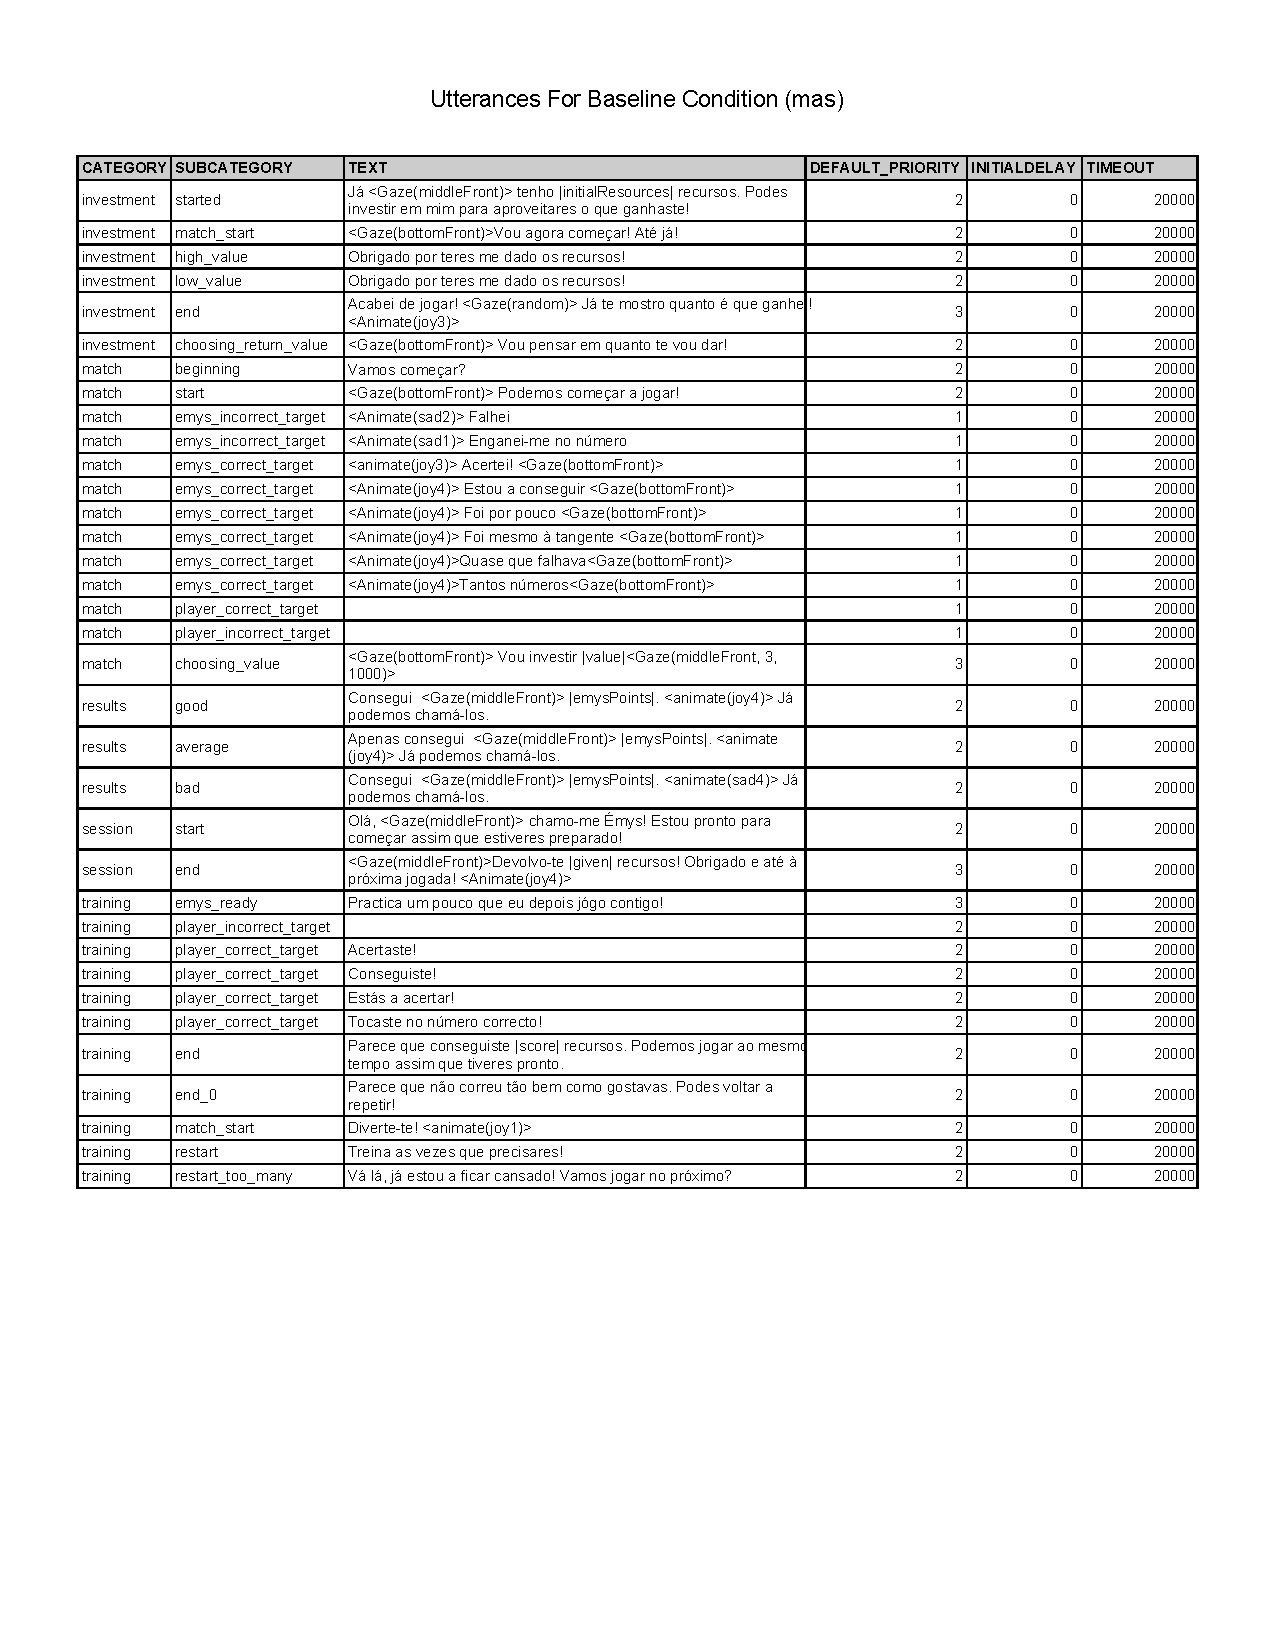
\includepdf[pages={-}]{external/UTTERANCES_BASELINE_mas.pdf}
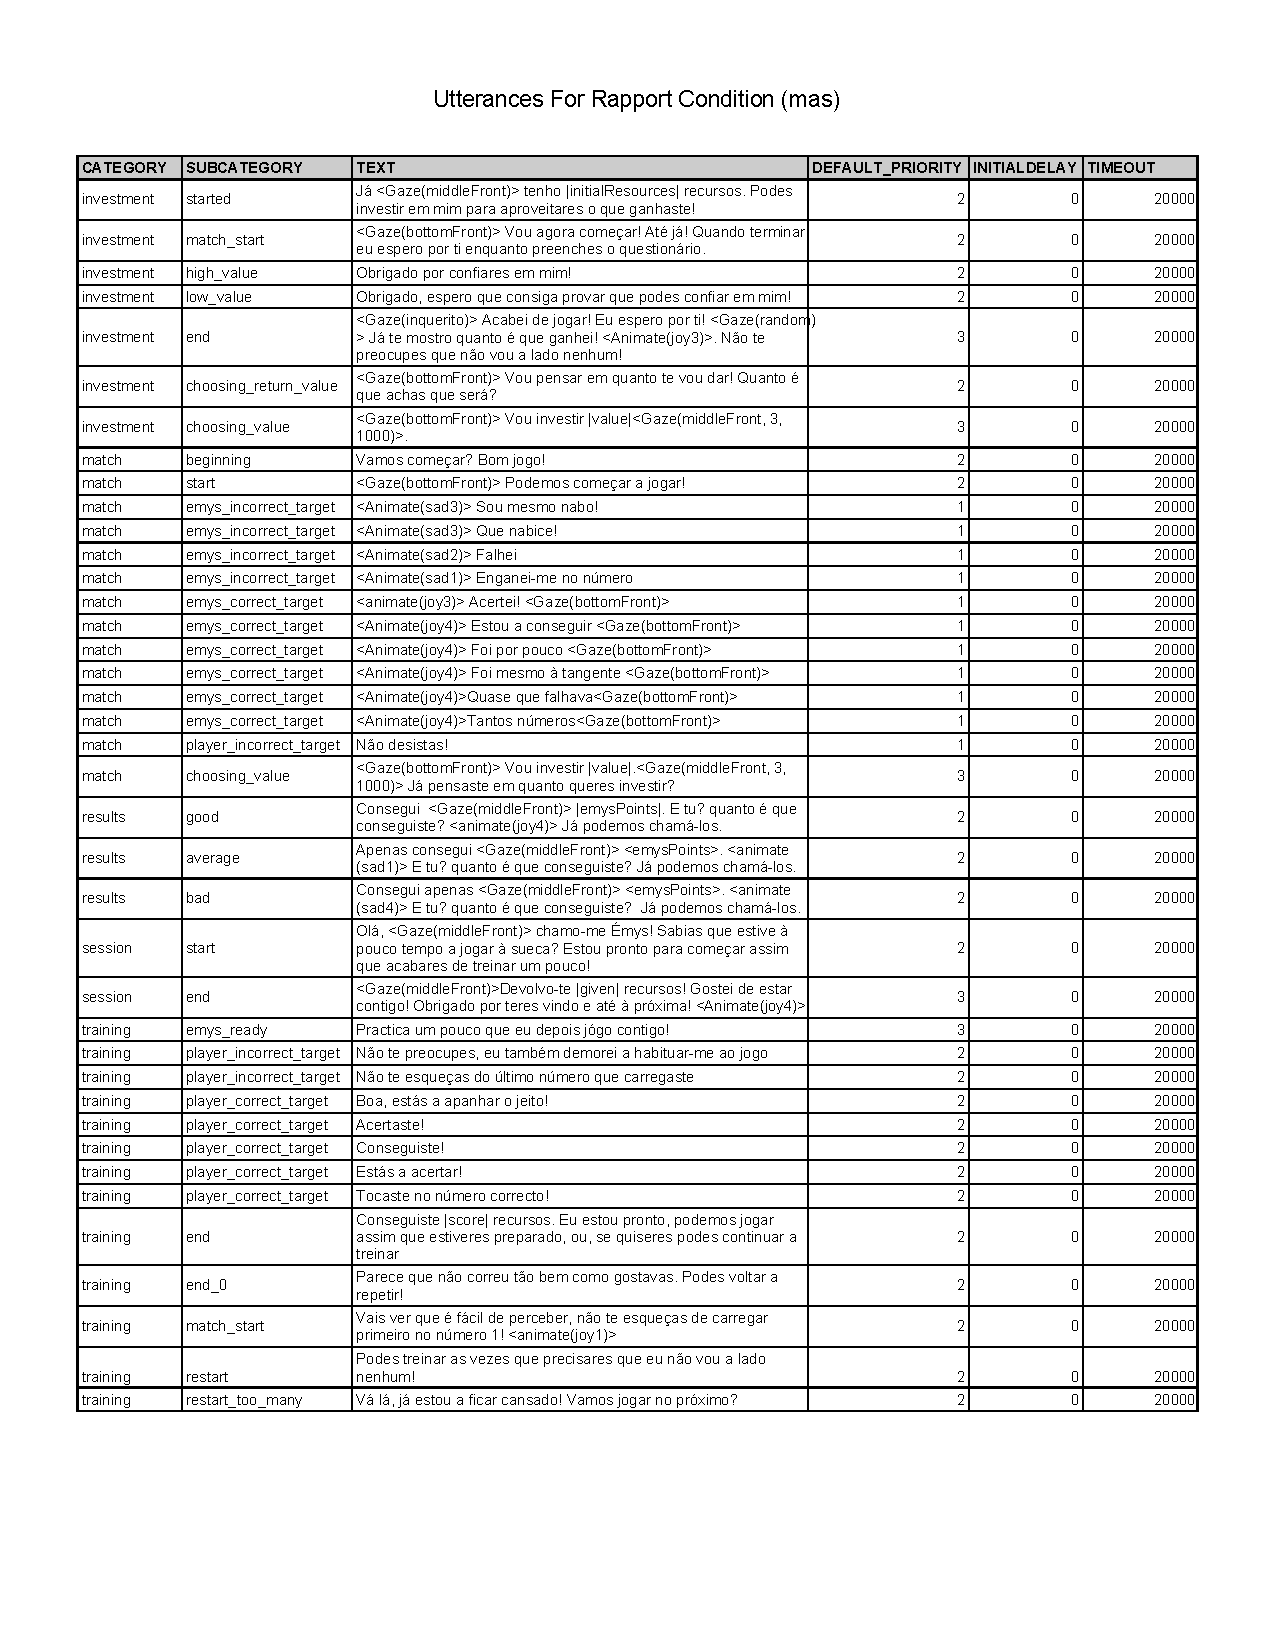
\includepdf[pages={-}]{external/UTTERANCES_RAPPORT_mas.pdf}
